\section{Simulation Environment}
\label{sect:simulation}

In order to experiment with robotic systems, a researcher requires a controllable robotic platform, a control system that interfaces to the robotic system and provides behaviors for the robot to carry out, and an environment to operate in. Our kitting application relies on an open source (the game engine is free, but license restrictions do apply), freely available framework capable of fulfilling all of these requirements. This framework is composed of the Unified System for Automation and Robot Simulation (USARSim) \cite{USARSimWeb} framework that provides the robotic platform and environment, and the Operating System (ROS)\footnote{Certain commercial software and tools are identified in this paper in order to explain our research. Such identification does not imply recommendation or endorsement by the authors, nor does it imply that the software tools identified are necessarily the best available for the purpose.}\cite{ROSWeb} framework that provides the control system.

\subsection{The USARSim Framework}

USARSim~\cite{CARPIN.LNAI.2006,WANG.WSC.2003} is a high-fidelity physics-based simulation system based on the Unreal Developers Kit (UDK)~\cite{UDKWeb} from Epic Games. USARSim was originally developed under a National Science Foundation grant to study Robot, Agent, Person Teams in Urban Search and Rescue~\cite{LEWIS.ICHC.2003}. Since that time, it has been turned into a National Institute of Standards and Technology (NIST)-led, community-supported open source project that provides validated models of robots, sensors, and environments.

%Altogether, the Karma Physics engine~\cite{KarmEngine} and high-quality 3D rendering facilities of the Unreal game engine allow the creation of realistic simulation environments that provide the embodiment of a robotic system. Furthermore, USARSim comes with tools to develop objects and environments (Unreal Editor) and it is possible to control actors in the game through a TCP/IP socket API.

Through its usage of UDK, USARSim utilizes the physX physics engine~\cite{physXWeb} and high-quality 3D rendering facilities to create a realistic simulation environment (Figure~\ref{3D_World}) that provides the embodiment of, and the environment for a robotic
system. The current release of USARSim consists of various model environments, models of commercial and experimental robots, and sensor models. High fidelity at low cost is made possible by building the simulation on top of a game engine. By delegating  simulation specific tasks to a high volume commercial platform (available for free to most users) which provides superior visual rendering and physical modeling, full user effort can be devoted to the robotics-specific tasks of modeling platforms, control systems, sensors, interface tools and environments. These tasks are in turn accelerated by the advanced editing and development tools integrated with the game engine. This leads to a virtuous spiral in which a wide range of platforms can be modeled with greater fidelity in a short period of time.

%USARSim was originally based upon simulated environments in the USAR domain. Realistic disaster scenarios as well as robot test methods were created (Figure~\ref{TestRoom}).
%Since then, USARSim has been used worldwide and more environments have been developed for different purposes. Other environments such as the NIST campus (Figure~\ref{3D_World-b}) and factories (Figure~\ref{3D_World-c}) have been used to test the performance of algorithms in different efforts~\cite{WANG.HFES.2005,BALAGUER.IROS.2008,KOOTBALLY.ITEA.2010}. The simulation is also widely used for the RoboCup Virtual Robot Rescue Competition \cite{RoboCupWeb}, the IEEE Virtual Manufacturing and Automation Challenge \cite{VMACWeb}, and has been applied to the DARPA Urban Challenge (Figure~\ref{3D_World-a}).

\begin{figure}[t!]
\centering
\subfigure[Test Room.]{\label{TestRoom}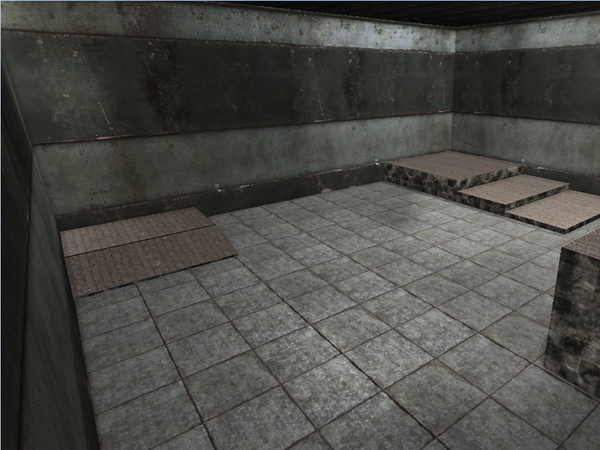
\includegraphics[width=4cm]{images/Worlds/testRoom.jpg}}\qquad
\subfigure[Factory,]{\label{3D_World-c}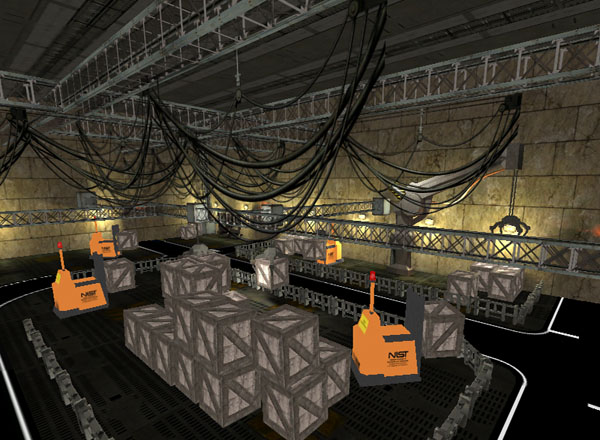
\includegraphics[width=4cm]{images/Worlds/factory.jpg}}
\caption{Sample of 3D environments in USARSim.} \label{3D_World}
\end{figure}

USARSim was initially developed with a focus on differential drive wheeled robots. However, USARSim's open source framework has encouraged wide community interest and support that now allows USARSim to offer multiple robots, including humanoid robots, aerial platforms (Figure~\ref{Fig:AirRobot}), robotic arms (Figure~\ref{Fig:KR60}), and commercial vehicles. In USARSim, robots are based on physical computer aided design (CAD) models of the real
robots and are implemented by specialization of specific existing classes. This structure allows for easier development of new platforms that model custom designs.

All robots in USARSim have a chassis, and may contain multiple wheels, sensors, and
actuators. The robots are configurable (e.g. specify types of
sensors/end effectors) through a configuration file that is read at run-time. The properties of the robots can
also be configured, such as the battery life and the frequency of
data transmission.

\begin{figure}[t!]
\centering
\subfigure[Air Robot AR100B.]{\label{Fig:AirRobot}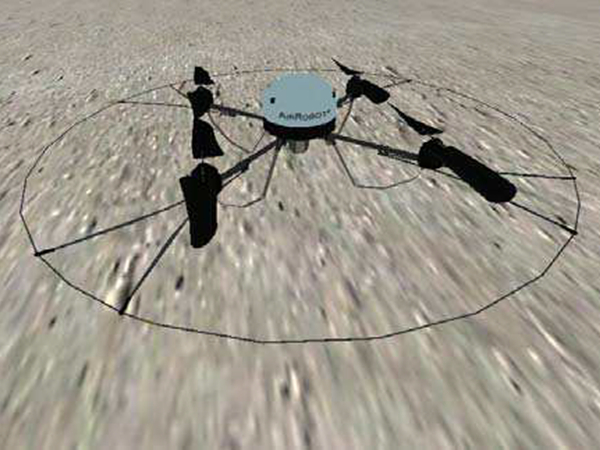
\includegraphics[width=4cm]{images/Robots/airRobot_2.jpg}}\qquad
\subfigure[Kuka KR60,]{\label{Fig:KR60}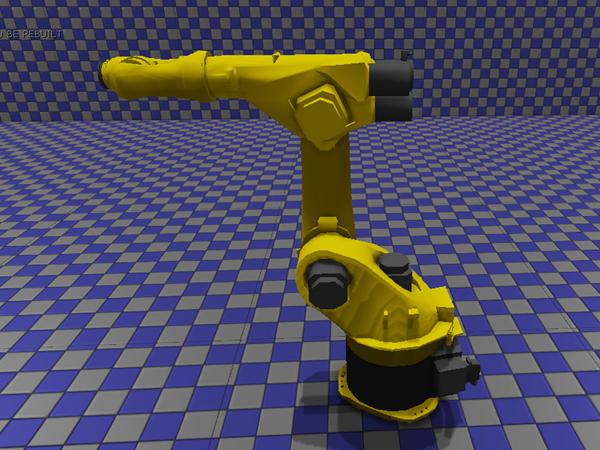
\includegraphics[width=4cm]{images/Robots/kr60.jpg}}
\caption{Sample of vehicles in USARSim.}
\end{figure}




\subsection{The ROS Framework}
ROS~\cite{ROSWeb} is an open source framework designed to provide an abstraction layer to complex robotic hardware and software configurations. It provides libraries and tools to help software developers create robot applications and has found wide use in both industry and academia. Examples of ROS applications include
Willow Garage's Personal Robots Program~\cite{WYOBEK.ICRA.2008} and the Stanford University STAIR project~\cite{QUIGLEY.AAAI.2007}. Developers of ROS code are encouraged to
contribute their code back to the community and to provide documentation and maintenance of their algorithms.

ROS possesses a large range of tools and services that both users and developers alike can benefit from. The philosophical goals of ROS include an advanced set of criteria and can be summarized as: peer-to-peer, tools-based, multi-lingual, thin, and free and open-source~\cite{QUIGLEY.ICRA.2009}. Furthermore, debugging at all levels of the software is made possible with the full source code of ROS being publicly available. Thus, the main developers of a project can benefit from the community and vice-versa.

In the effort described in this paper, the authors have used ROS as the main system controller. Once a CRCL plan file is generated by the interpreter from the PDDL plan file (Robot Language level in Figure~\ref{fig:methodology}), the CRCL plan file is parsed by the ROS controller and each robot command in this file is executed by the simulated robotic arm.

